%% This is an example first chapter.  You should put chapter/appendix that you
%% write into a separate file, and add a line \include{yourfilename} to
%% main.tex, where `yourfilename.tex' is the name of the chapter/appendix file.
%% You can process specific files by typing their names in at the 
%% \files=
%% prompt when you run the file main.tex through LaTeX.
\chapter{Design}

In this chapter we argue all design decisions taken regarding the building of Redch. These are grounded on the detailed research explained in Chapter 3. It extends the high-level architecture already outlined in \ref{fig:use_cases} further by first explaining the technology used: the programming languages, frameworks and most relevant libraries. Then, it presents the whole architecture of the system by describing each one of the components the system is comprised of.

The design explained below aims to be a solid ground and a first prototype for the Redch project. Therefore, not all ideas discussed in previous chapters may be included in the result of this master thesis. As a first step towards the final product it will serve to get insight...

Ruby has been chosen as the main language for the development of the project. This dynamic language focused on simplicity and productivity, is often regarded as developer performant. Due to its flexibility and similarity with natural language, along with the massive amount of libraries and frameworks available, it allows developers to write applications very quickly. However, this features hamper its execution performance.

\subsection{Physical Architecture}

The core idea of this architecture is to decouple the data producers from the data consumers by means of an asynchronous message queue enabling push capabilities in the consumption tier. It is compound of four different servers, as figure \ref{fig:physical_architecture} shows: An application server that receives the observations from the sensors and stores them in the database. That server is also responsible for publishing the observation into the messaging queue. Then, the messaging queue pushes them to the data consumption tier, where the app server sends them to the web clients.

Doing so, implies a number of benefits as outlined in Chapter 3. First and foremost, each tier can easily scale out independently. For both tiers, the throughput can be increased adding more app servers. As for the database and the messaging queue, clusterizing them can provide better performance, increased throughput and storage capacity.

The loosely coupled architecture the messaging queue entails not only allows scaling horizontally, but also allows components to evolve independently. The only constraint is that both tiers must understand the Advanced Message Queuing Protocol (AMQP). On the other hand, given the wide adoption of such protocol, the particular messaging queue may be replaced without affecting any of the tiers.

Finally, a high-performance asynchronous messaging queue provides real-time capabilities to the system.

\begin{figure}[ht]
	\centering
	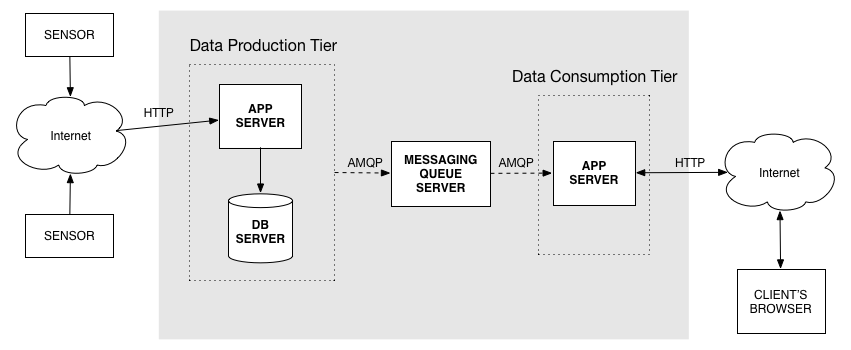
\includegraphics[width=\textwidth]{physical_architecture}
	\caption{Physical Architecture}
	\label{fig:physical_architecture}
\end{figure}

\subsection{Logical Architecture}

To start with, given the CREAF's determination towards the SWE initiative and involvement in Open-source GIS community it is important to make use of the Sensor Observation Service (SOS). To do so, we opt for 52ºNorth SOS 4.0, the leading open-source SOS implementation already integrated by many research institutions throughout the world. In this regard, great efforts are underway to bring last web standards to the OGC implementations, which may be worth checking out in order to include them in Redch project. This is the case of 52ºNorth SOS 4.0. While this project uses its beta version, the final version has been released less than three months as of this writing.




Nonetheless, usually message queues aren't the system's bottleneck, but message consumers slowed down by database queries or backend systems.

impact on client of AMQP, SSE. Async app server. Reactor pattern.

\subsection{Database}

To that end, it must be taken into account the pattern of the data flow.
  
Ever growing data set, very small data units and mainly write ops.


NoSQL
MongoDB most mature

cons: 
- migration from relational design
